% !TEX TS-program = pdflatex
% !TEX encoding = UTF-8 Unicode

% This is a simple template for a LaTeX document using the "article" class.
% See "book", "report", "letter" for other types of document.

\documentclass[11pt]{article} % use larger type; default would be 10pt

\usepackage[utf8]{inputenc} % set input encoding (not needed with XeLaTeX)

%%% Examples of Article customizations
% These packages are optional, depending whether you want the features they provide.
% See the LaTeX Companion or other references for full information.

%%% PAGE DIMENSIONS
\usepackage{geometry} % to change the page dimensions
\geometry{a4paper} % or letterpaper (US) or a5paper or....
% \geometry{margin=2in} % for example, change the margins to 2 inches all round
% \geometry{landscape} % set up the page for landscape
%   read geometry.pdf for detailed page layout information

\usepackage{graphicx} % support the \includegraphics command and options

% \usepackage[parfill]{parskip} % Activate to begin paragraphs with an empty line rather than an indent

%%% PACKAGES
\usepackage{booktabs} % for much better looking tables
\usepackage{array} % for better arrays (eg matrices) in maths
\usepackage{paralist} % very flexible & customisable lists (eg. enumerate/itemize, etc.)
\usepackage{verbatim} % adds environment for commenting out blocks of text & for better verbatim
\usepackage{subfig} % make it possible to include more than one captioned figure/table in a single float
% These packages are all incorporated in the memoir class to one degree or another...

%%% HEADERS & FOOTERS
\usepackage{fancyhdr} % This should be set AFTER setting up the page geometry
\pagestyle{fancy} % options: empty , plain , fancy
\renewcommand{\headrulewidth}{0pt} % customise the layout...
\lhead{}\chead{}\rhead{}
\lfoot{}\cfoot{\thepage}\rfoot{}

%%% SECTION TITLE APPEARANCE
\usepackage{sectsty}
\allsectionsfont{\sffamily\mdseries\upshape} % (See the fntguide.pdf for font help)
% (This matches ConTeXt defaults)

%%% ToC (table of contents) APPEARANCE
\usepackage[nottoc,notlof,notlot]{tocbibind} % Put the bibliography in the ToC
\usepackage[titles,subfigure]{tocloft} % Alter the style of the Table of Contents
\renewcommand{\cftsecfont}{\rmfamily\mdseries\upshape}
\renewcommand{\cftsecpagefont}{\rmfamily\mdseries\upshape} % No bold!

%%% END Article customizations

%%% The "real" document content comes below...

\title{Tetris with Gravity - Project Specification}
\author{Nordberg, Marcus \\ mnordber@kth.se
		\and
	Rolleberg, Niklas \\ nrol@kth.se}
%\date{} % Activate to display a given date or no date (if empty),
         % otherwise the current date is printed 

\begin{document}
\maketitle

\section{Background}
Tetris is a very classic game and it is very easy to get into. However, it severely lacks in the physics department. The movement of the bricks is unrealistic and this is what this project intends to fix.

Similar projects has been done in the past. This is taken from the YouTube video ``Let's Not Play Tetris''\footnote{https://www.youtube.com/watch?v=SMXmFF2hoY4}. Our implementation will be different in the aspect that we intend to let gravity accelerate the brick and they will also be pretty elastic so that they will bounce off eachother.
\begin{center}
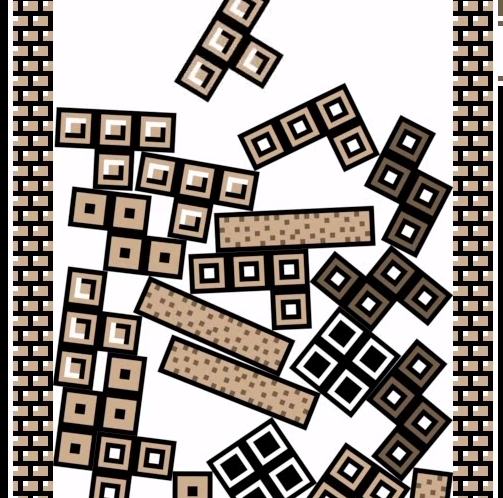
\includegraphics[scale=0.5]{tetris-gravity}
\end{center}

\section{Problem}
This project will introduce physics into the world of Tetris. Bricks will be affected by gravity and collision will be brutal to the bricks. This will of course make the game unwinnable as the player won't be able to get a full line.

Due to the time constraint, the game will probably be pretty limited. One thing we might do to make it easier is to fix the bricks who has fallen. Instead of having update all of the bricks at collision, just the currently active brick will bounce around and act upon the laws of physics.

\section{Implementation}
As the time is limited we will probably do this project in Python because we're both familiar with the language. We will probably use a game module like PyGame\footnote{http://pygame.org/} to speed up the development process.

\section{Evaluation}
It is hard to evaluate a game like Tetris. Our hope is that this will be a fun demonstration and that it will lead to much frustration for the player. We intend to not tell the audience about the twist before demonstrating the game so it will hopefully be a fun surprise.
\end{document}
